\section{Purpose and Coupling}
With these concepts defined by \citeA{norman} there is a strong foundation for creating a game design framework, however, these concepts focus solely on communicating how something works: "You can figure out the scissors because their operating parts are visible and the implications clear. The conceptual model is obvious, and there is an effective use of signifiers, affordances, and constraints" \cite[p. 27]{norman}. But how does one realise that a scissor is for cutting paper? \citeA{norman} does not describe how a design can communicate its purpose. Furthermore, when \citeA{norman} writes that the fact that a scissor's operating parts are visible is what makes the scissor intuitive, an interesting point is made but is not further explored in \citeA{norman}. In \citeA{normanold}, the reason for what makes the scissors intuitive could be described by the concept of \textit{visibility}, but this concept seems to have been incorporated into the more general concept of signifiers. \citeA{howdonald} and \citeA{frogger} offer a more detailed explanation with their definitions of \textit{feedforward} and \textit{feedback} with their subdivisions \textit{inherent, augmented} and \textit{functional}. I will describe their definitions and delve into their definitions of these two concepts in correlation to the concepts of \citeA{norman} because they themselves consider the concepts as building on top of the notions of \citeA{normanold}, and because Norman's concepts have been revised \cite{norman} after the fact. A major revision to regard is the addition of the concept of signifiers and the alteration of the definition for affordances. \citeA{norman} notes about affordances that "[a]las, the term became used in ways that had nothing to do with the original" \cite[p. 13]{norman}. He argues that the design community understood the term as a property instead of a relationship when it needed a term to describe the addition of instructional elements. Therefore, signifiers were termed and affordances were made more concrete. The more broad understanding of affordances is, therefore, the one that is present in \citeA{howdonald} and \citeA{frogger}. However, the arguments and definitions are still relevant for the bolstering of my design framework, since the insights made, do not overlap directly with the old or new insights of \citeA{norman}, but instead expand the research field.

\subsection{Feedforward} Feedforward is the information an object gives before an interaction, about what the consequences of an action will be. This is given both by the way the object looks, but also the action that it requires \cite{frogger}. It adds on perceivable affordances in the way that feedforward also informs about what the results of a user's action will be, i.e. the purpose of an action \cite{vermeulen}. To further describe the concept of feedforward, \citeA{frogger} divide the concept into three subdivisions: inherent, augmented and functional.
\paragraph{Inherent Feedforward} Resembles perceivable affordances \cite{norman} in the sense that it communicates the action possibilities of the design through the relationship between the user and the design. Additionally, inherent feedforward communicates how this action can be made (rotating, pushing, pulling, etc.) and what the consequence of that action will be \cite{frogger}. It is, importantly, part of the interaction, thereby making the information inherent to the interaction. This will mean that the information is also stemming from the location of the interaction. As a consequence of it being inherent to the physical interaction, it appeals to the perceptual-motor skills of the user \cite{frogger}.
\paragraph{Augmented Feedforward} Communication about the action possibilities and the purpose of the action coming from an additional source \cite{frogger}. As an example, a lit button next to an elevator shaft communicates to the awaiting future passengers that the car will make a stop at this floor. The light inside or next to the button would be augmented feedforward since it is remote from the actual elevator car, but gives information about the goal of the future passengers: to enter the elevator. This kind of information, thusly, relies on the user's cognitive abilities since it is the user that needs to know that the light near or on the button indicates that the elevator will stop at his or her floor. This, \citeA{norman} describes as a signifier.
\paragraph{Functional Feedforward} Functional feedforward communicates the general purpose of the design, i.e. why to do the action \cite{frogger}. Functional feedforward can utilise the concept of \textit{product semantics} \cite{semantics}, where the user's previous experience is relied upon for her to find meaning in the design. Additionally, as described in the scissor example from earlier, functional feedforward can describe the communication that happens when the operating parts are visible to the user, thereby making the function clear \cite{frogger}.

In \citeA{howdonald}, the application of feedforward is explained as follows: The designer must create meaning for the user, and for this, there are two approaches: the semantic approach and the direct approach \cite{howdonald}. These two approaches are what later in \citeA{frogger} can be described as providing functional information through augmented information and inherent information. The semantic approach providing augmented information and the direct approach providing inherent information. More on this will be discussed in the coupling section. The semantic approach relies on the user's previous experiences and applies that to inform the user of its own resemblance to that previous experience. It often benefits from the use of iconography and symbols \cite{howdonald}. This approach resembles signifiers, and a product of this approach could presumably be interpreted as both a signifier and augmented feedforward. 2) The direct approach instead, relies only on bodily and perceptual skills and the intention being that meaning should be created in the interaction. Since perceptual and bodily skills are relied upon, the approach requires tangible interaction \cite{howdonald}. The approach utilises the concept of natural mapping because of the way the spatial layout of a design can communicate the purpose of an action. Spatial layout, however, is just one utilisation of this approach. \citeA{howdonald} describe an example of this approach where part of a design is used to silence the sound it emits: The operating part is placed on top of where a loudspeaker is emitting the sound from, and the loudspeaker is thereafter silenced. The purpose of this action is communicated naturally since it is common knowledge that placing a physical object on top of something that emits sound, obstructs the sound being emitted.

For applying feedforward in a design, \citeA{howdonald} argue that the direct approach should be prioritized. It takes behaviour and action as its starting point and instead of focusing on semantics where cognitive skills are relied on to find meaning in resemblance, the authors believe that meaning is created in the interaction and, thereby, relying on perceptual and bodily skills put less strain on the user. An argument that is echoed later in \citeA{frogger}.

\subsection{Feedback} The definition of feedback in \citeA{frogger} is similar to that of \citeA{norman}. Similarly to feedforward, \citeA{frogger} divides feedback into the three subdivisions of functional, augmented and inherent.
\paragraph{Functional Feedback} The feedback the user receives concerning the desired functionality from a design \cite{frogger}. If the user flickers a light switch to turn on a light, a light turning on would be the functional feedback.
\paragraph{Augmented Feedback} This is feedback coming from an additional source \cite{frogger}. In the elevator example from earlier, the button that lights up when pressed would be augmented feedback, communicating that the car will stop on the indicated floor. The actual consequence of the car stopping on the desired floor would be functional feedback.
\paragraph{Inherent Feedback} Inherent feedback means that the performed action and the feedback it gives are closely coupled. The inherent feedback of an action acts as an innate consequence of that action. Unlike augmented feedback, inherent feedback comes from the action itself. The feedback appeals to the perceptual-motor skills of the user and can be received visually, auditorily and haptically \cite{frogger}.

\subsection{Coupling}
Consider the scissor example from earlier once more: When operating a scissor the feedback the user receives is through all of her perceptual motor skills: The incision point of the blades and the paper is visible, the sound of the paper splitting is heard, the haptic feel of the resistance is felt and the blades follow the motion of your hand and fingers. This close coupling of action and meaning is logically always apparent in mechanical products and makes them intuitive because action and meaning are unified on the six aspects of time, location, direction, dynamics, modality and expression through inherent information \cite{frogger} \cite{transbehav}:
\begin{itemize}
  \item \textit{Time}: The action and meaning take place at the same time.
  \item \textit{Location}: The action and meaning take place at the same place.
  \item \textit{Direction}: The direction of the action and meaning is the same.
  \item \textit{Dynamics}: The speed, acceleration and force of the action is closely coupled to the speed, acceleration and force of the meaning.
  \item \textit{Modality}: The sensory modalities (appearance, sound, taste, feel, etc.) of the action are mirrored in the meaning.
  \item \textit{Expression}: Any expression is apparent in both the action and the meaning.
\end{itemize}

Electronic products, \citeA{frogger} argues, can take advantage of these six aspects of coupling to make the interaction more intuitive by coupling the action and function through augmented and inherent information. What electronic products lack, is the direct coupling between action and function through inherent information that a scissor as an example would have. To illustrate how a design can be regarded through these six aspects, I will return to the elevator setting, instead, now the user is inside the elevator car. Here the action would be the pushing of a button with the intent of directing the elevator car to the indicated floor, and the function, being transported to that floor.
\paragraph{Time} The action of pushing the button and actually arriving at that floor does not take place at the same time, however, as is often the case in elevators, augmented information is used to indicate the compliance of the desired function; this is often done by lighting a light near or on the button and this occurs at the same time as the action. Action and meaning are therefore coupled with the aspect of time through augmented information.
\paragraph{Location} The action of pushing the button and the destination floor is not at the same location, however, a light that lights up on the button to indicate its compliance, is in the same location as the action. Action and meaning are therefore coupled with the aspect of location through augmented information. As \citeA{frogger} also mentions, the aspect of location being communicated through augmented information is the equivalent of mapping from \citeA{normanold}.
\paragraph{Direction} The direction of the button push and the transportation direction is not the same: One is horizontal, the other vertical. Here, the augmented information offers no coupling, and thusly, action and meaning are not coupled on the aspect of direction. One way of providing a coupling on this aspect would be to replace the button interface with an interface that allows for swiping gestures; then instead of pushing the desired button, a user would swipe from a graphic representing the current floor to a graphic representing the desired floor. The action, i.e. the swipe, would then be in the same direction as the transportation, thereby coupling action and function through augmented and inherent information. Inherent because the information about the directions stems from the action itself, and augmented because the action takes place at an additional source (the interface).
\paragraph{Dynamics} The speed, acceleration and force of the button push are not apparent in the speed, acceleration and force of the transportation. Augmented information also does not offer any coupling, and action and meaning are thusly not coupled on the aspect of dynamics. An inspiration for a possible iteration, to couple action and meaning on this aspect, could be taken from the real world, where a rushed user can be seen rapidly pushing a button with the hope that the rapid pushes can accelerate the transport. If the proposal of the busy elevator user were to be implemented, the elevator would be coupled on the aspect of dynamics through augmented and inherent information. Inherent because the information about the dynamics stems from the action itself, and augmented because the action takes place at an additional source (the elevator car).
\paragraph{Modality} The sensory modalities of the button push are not mirrored in the transportation. There is little to no link between the appearance, sound, feel, etc. of the action and the function of an elevator. A vague argument can be made that having square buttons could resemble the shape of the elevator car, thereby coupling action and meaning on the aspect of modality (the appearance) through augmented information. A stronger coupling could be made with for example sound: Pushing a button emits a specific tone; the higher the floor, the higher the tone. The elevator car constantly hums a tone; the higher the floor it is on, the higher the tone. Then, as the elevator progresses the floors toward the desired floor, the hummed tone nears the tone from the button press i.e. the tone of the floor.
\paragraph{Expression} No expression is apparent in both the button push and the transportation. No matter how furiously you hammer the button, the elevator car will transport you the same way as if you had playfully tickled the button. The elevator offers no coupling between action and meaning on the aspect of expression. However, using the hurried elevator user from earlier, it is apparent that such a design is possible. The expression of the user's rapid button press, with the desire for the transportation to hurry, is a hectic, frantic one. A way for the transportation to reflect this is to first transport the user at a hurried pace, but also more imprecise. The doors could open asynchronously or the elevator car can stop at a point that is less level with the floor than we would otherwise expect. With this design implemented the elevator would be coupled on the aspect of expression through augmented and inherent information. Inherent because the information about the expression stems from the action itself, and augmented because meaning takes place at an additional source (the elevator doors and car).

\begin{figure}[h]
  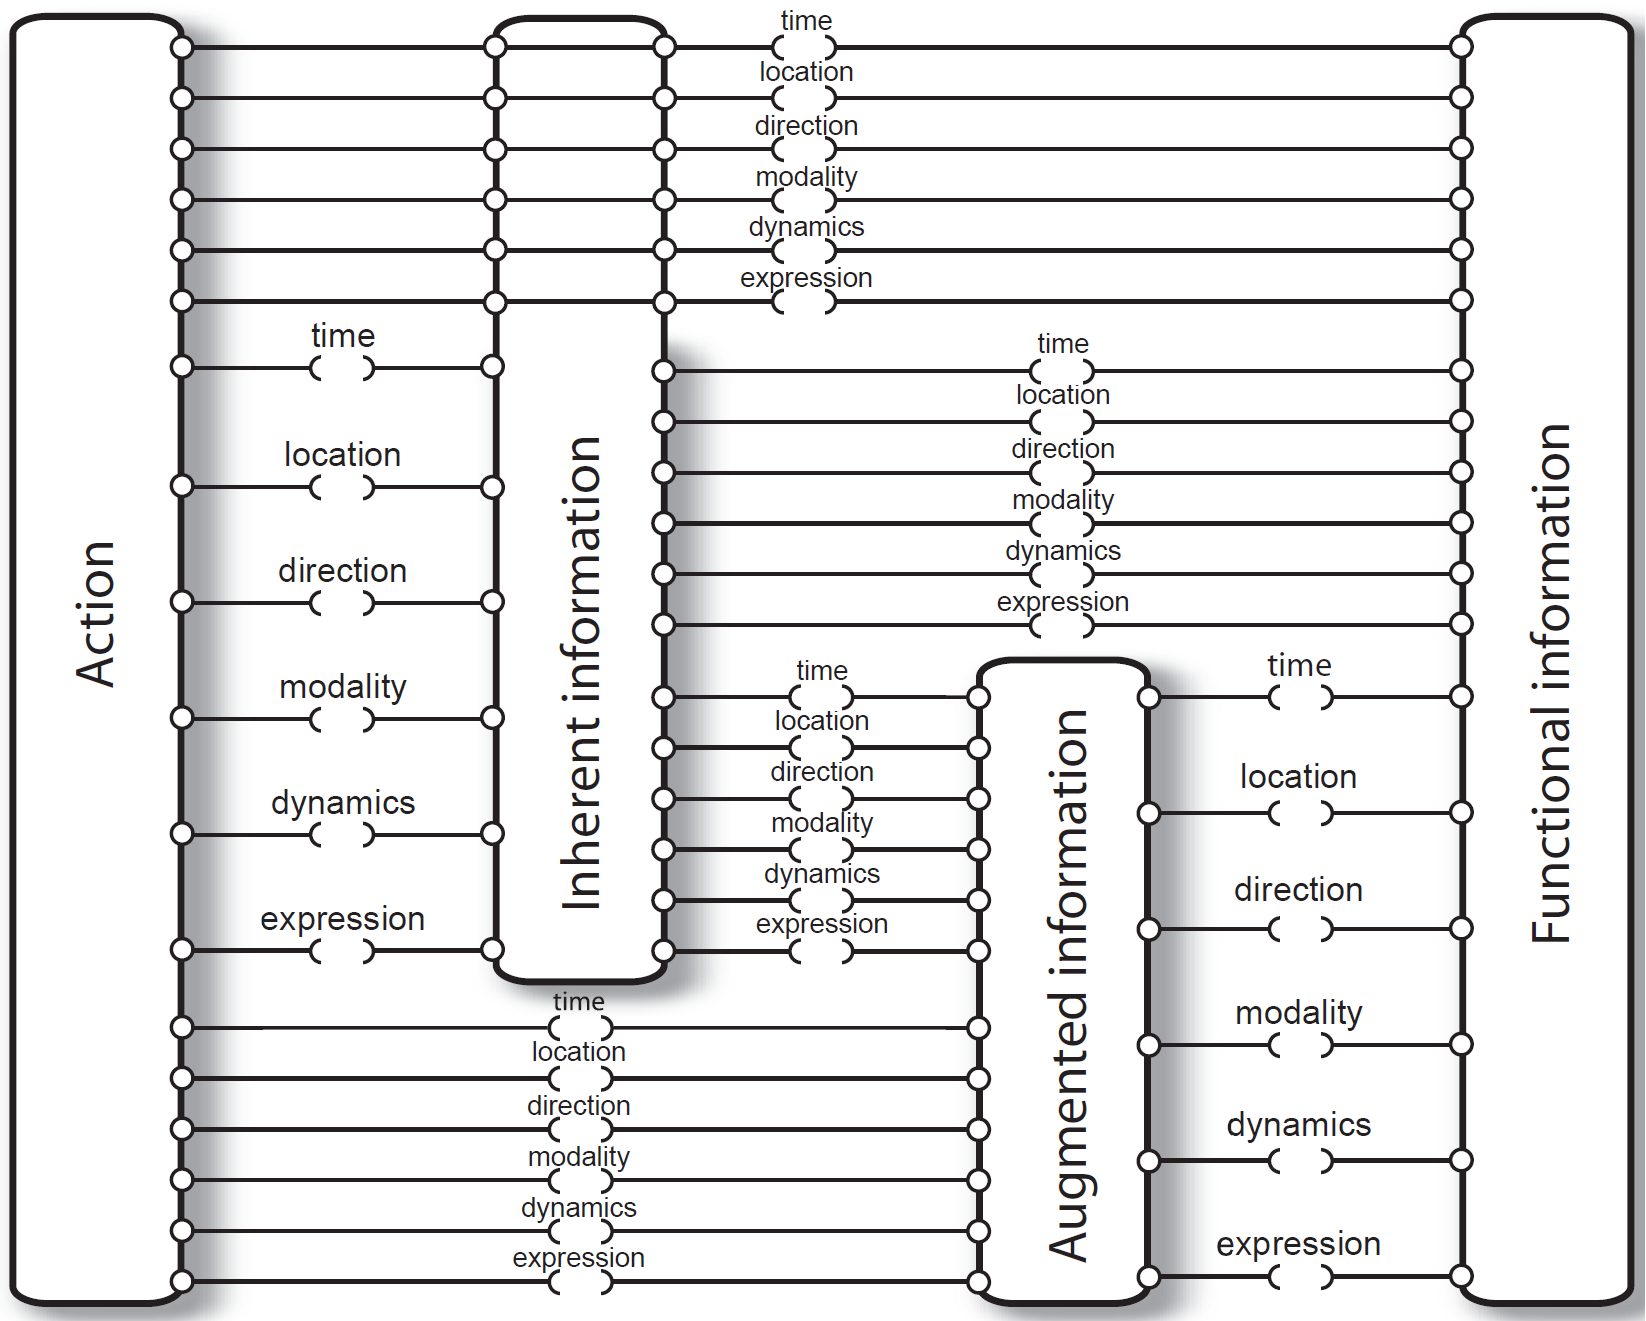
\includegraphics[width=\textwidth]{FroggerDefault}
  \caption{The Frogger Framework}
  \label{frogdef}
\end{figure}

From these two information directions (feedforward and feedback) with three subdivisions (functional, inherent and augmented) and six aspects to couple them on (time, location, direction, modality, dynamics and expression), \citeA{frogger} formulated a framework called the Frogger Framework (see figure \ref{frogdef}). The framework is a "[...] A schematic interpretation of all the different coupling possibilities between the functional information and the user’s action" \cite[p. 6]{frogger}. This schematic approach has a high amount of complexity, which could explain why others have chosen to simplify the model \cite{tangifrog} and why \citeA{transbehav}, who include Stephan Wensveen, see an altered and simplified model as "[...] more useful" \cite[p. 22]{transbehav}. The altered and simplified version is also the version I will refer to henceforth (see figure \ref{frogalt}).

\begin{figure}[h]
  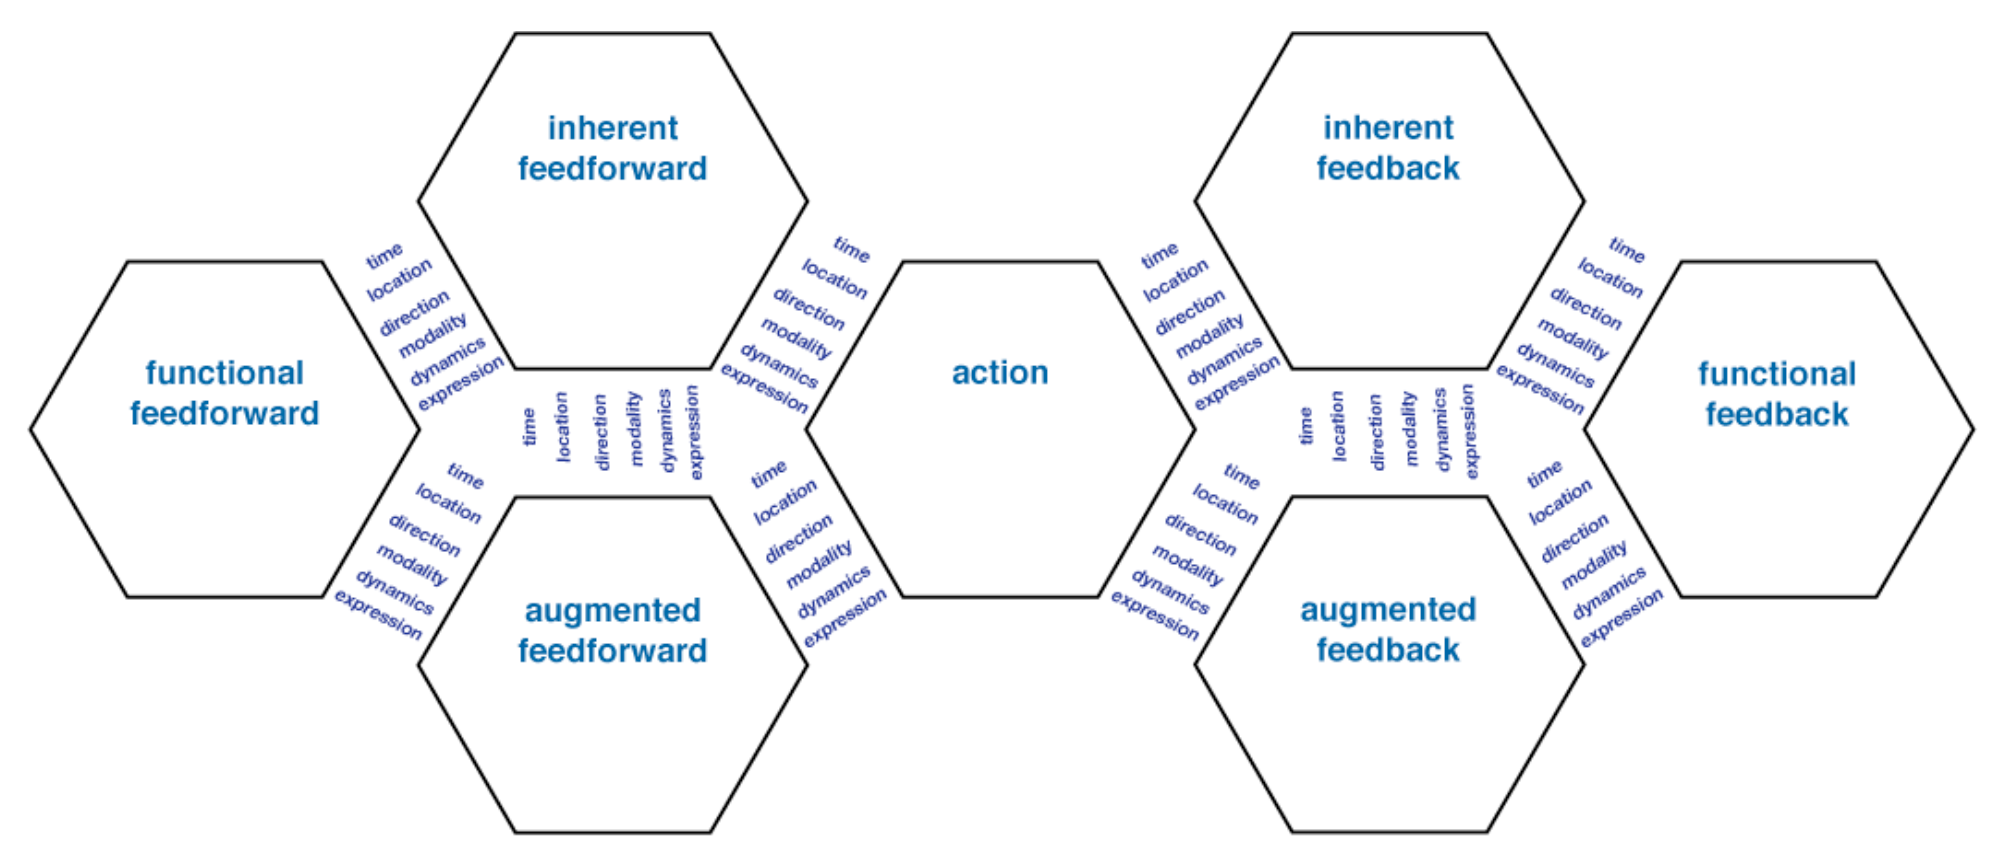
\includegraphics[width=\textwidth]{FroggerAlt}
  \caption{The Alternate Frogger Framework}
  \label{frogalt}
\end{figure}

\newpage
